\documentclass{beamer}

\usetheme{metropolis}

\usepackage{xparse}
\usepackage{xfrac}
\usepackage[siunitx, american]{circuitikz}
\usepackage{hyperref}
\usepackage{cancel}
\usepackage{amssymb}
\usepackage{amsmath}
\usepackage{graphicx}
\usetikzlibrary{automata, arrows}

% https://tex.stackexchange.com/questions/2233/whats-the-best-way-make-an-augmented-coefficient-matrix
\makeatletter
\renewcommand*\env@matrix[1][*\c@MaxMatrixCols c]{%
  \hskip -\arraycolsep
  \let\@ifnextchar\new@ifnextchar
  \array{#1}}
\makeatother


% https://tex.stackexchange.com/questions/102069/make-a-heading-in-beamer
\newcommand\makeheader[1]{%
  \par\bigskip
  {\large\bfseries#1}\par\smallskip}

\title{EECS 16A Midterm 1 Review Session}
\author{Presented by \textless NAMES \textgreater (HKN)}
\date{}




\begin{document}

\begin{frame}

\titlepage

\end{frame}

\begin{frame}[t]\vspace{20pt}
\frametitle{Disclaimer}
Although some of the presenters may be course staff, the material covered in the review session may not be an accurate representation of the topics covered in and difficulty of the exam.

\vspace{20pt}
Slides are posted at --- on Piazza.

\end{frame}


\begin{frame}[t]\vspace{20pt}
\frametitle{HKN Drop-In Tutoring}

\begin{itemize}
\item These details should be edited
\end{itemize}

\end{frame}

\section*{Systems of Equations and Gaussian Elimination}

\begin{frame}[t]\vspace{20pt}
\frametitle{Vectors}
Conceptually, a vector is a collection of numbers that each represent a variable. If there are $n$ variables, then the vector is $n$-dimensional.

Example: \newline
A point in 3D can be represented as $(x,y,z)$
In vector form, this would be represented as $\begin{bmatrix} x \\ y \\ z \\ \end{bmatrix}$

\end{frame}


\begin{frame}[t]\vspace{5pt}
\frametitle{Matrices}
\begin{itemize}
\item Collection of \textbf{vectors}
\item 2D table for \textbf{storing data}
	\begin{itemize}
		\item[$\circledcirc$] Systems of equations for imaging observations
	\end{itemize}
\item Notable/useful matrices
	\begin{itemize}
		\item[$\circledcirc$] Identity matrix
		\item[$\circledcirc$] Augmented matrices
		\item[$\circledcirc$] Rotation matrix
		\item[$\circledcirc$] Many others!
	\end{itemize}
\end{itemize}

Augmented:
$\begin{bmatrix}[ccc|c]
1 & -2 & 3 & 7\\
2 & 1 & 1 & 4\\
-3 & 2 & 3-2& 10\\
\end{bmatrix}$

Rotation: \hspace{9pt}
$\begin{bmatrix}
\cos{\theta} & -\sin{\theta} \\
\sin{\theta} & \cos{\theta} \\

\end{bmatrix}$

\end{frame}



\begin{frame}[t]\vspace{10pt}
\frametitle{Matrix Transformations}

Matrices are often used to perform transformations, especially 
\newline in $\mathbb{R}^2$ \\~\\
Two important transformations:

\begin{figure}[!tbp]
  \centering
  \begin{minipage}[b]{0.3\textwidth}
    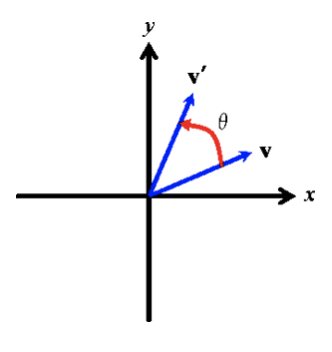
\includegraphics[width=\textwidth]{./images/rotation.png}
    \caption{Rotation}
  \end{minipage}
  \hfill
  \begin{minipage}[b]{0.3\textwidth}
    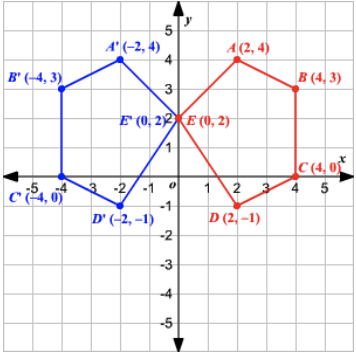
\includegraphics[width=\textwidth]{./images/reflection.png}
    \caption{Reflection}
  \end{minipage}
\end{figure}
\end{frame}



\begin{frame}[t]\vspace{10pt}
\frametitle{Rotation Matrix}
The rotation matrix rotates points by a specified angle, theta: \\~\\
$R(\theta) = \begin{bmatrix}
\cos{\theta} & -\sin{\theta} \\
\sin{\theta} & \cos{\theta} \\
\end{bmatrix}$

Use this matrix by plugging in desired rotation angle, then multiply with vector. \\
\textbf{Note: } Rotation matrices also preserve the length of a vector. \\~\\
\textbf{Example}: Rotation Matrix that rotates vector by $90^{\circ}$ \\~\\
$R(90^{\circ}) = \begin{bmatrix}
0 & -1 \\
1 & 0 \\
\end{bmatrix}$
\end{frame}

\begin{frame}[t]\vspace{10pt}
\frametitle{Rotation Matrix}
The rotation matrix rotates points by a specified angle, theta: \\~\\
$R(\theta) = \begin{bmatrix}
\cos{\theta} & -\sin{\theta} \\
\sin{\theta} & \cos{\theta} \\
\end{bmatrix}$

Use this matrix by plugging in desired rotation angle, then multiply with vector. \\
\textbf{Note: } Rotation matrices also preserve the length of a vector. \\~\\
\textbf{Example}: Rotation Matrix that rotates vector by $90^{\circ}$ \\~\\
$R(90^{\circ}) = \begin{bmatrix}
0 & -1 \\
1 & 0 \\
\end{bmatrix}$
\end{frame}

\begin{frame}[t]\vspace{10pt}
\frametitle{Reflection Matrix}

The reflection matrix reflects vectors across a line (Notice that such matrix also preserves the length of a vector)\\~\\
Notable reflection matrices:

\begin{figure}
  \begin{minipage}{.5\linewidth}
    \centering
    \[\left[\begin{array}{cc}
      1 &  0\\
      0 & -1
    \end{array}\right]\]
    Reflection across $x$-axis
  \end{minipage}%
  \begin{minipage}{.5\linewidth}
    \centering
    \[\left[\begin{array}{cc}
      -1 &  0\\
      0 & 1
    \end{array}\right]\]
    Reflection across $y$-axis
  \end{minipage}
  \begin{minipage}{.5\linewidth}
    \centering
    \[\left[\begin{array}{cc}
      0 & 1\\
      1 & 0
    \end{array}\right]\]
    Reflection across $y=x$
  \end{minipage}
\end{figure}
\end{frame}



\begin{frame}[t]\vspace{10pt}
\frametitle{Matrix Transformations}
All linear transformations can be expressed as a matrix

\begin{figure}[!tbp]
  \centering
  \begin{minipage}[b]{0.45\textwidth}
    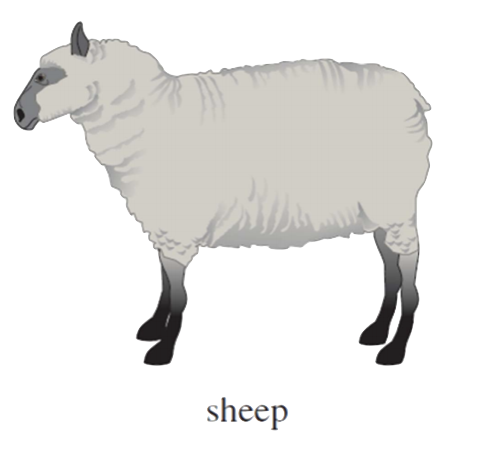
\includegraphics[width=\textwidth]{./images/sheep.png}
  \end{minipage}
  \hfill
  \begin{minipage}[b]{0.45\textwidth}
    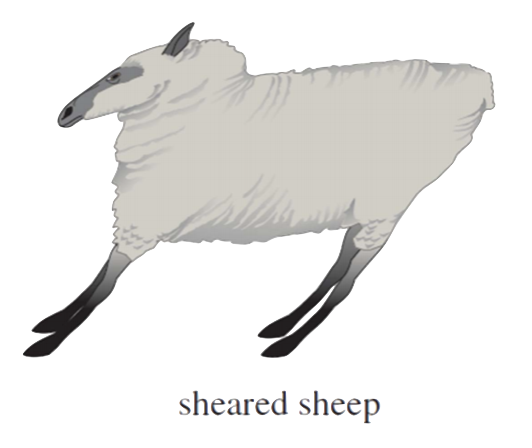
\includegraphics[width=\textwidth]{./images/sheep_shear.png}
  \end{minipage}
\end{figure}
\end{frame}


\begin{frame}[t]\vspace{-10pt}
\frametitle{Example 1}
\only<1>{\makeheader{Question}}
\only<2>{\makeheader{\textcolor{red}{Solution}}}

What is the resulting vector after the following (non-subsequent) transformations are applied 
to the vector 
$\vec{v}= \begin{bmatrix}
2 \\ 3
\end{bmatrix}$
\\~\\

\begin{enumerate}
\setcounter{enumi}{0}
\item Rotate by $45^{\circ}$
\end{enumerate}

\only<1>{\vspace{30pt}}

\only<2>{
\vspace{-10pt}
\[
\begin{bmatrix}
    \cos{45^{\circ}}  &  -\sin{45^{\circ}}      \\
    \sin{45^{\circ}}  &  \cos{45^{\circ}}    
\end{bmatrix}
= 
\begin{bmatrix}
    \frac{\sqrt{2}}{2}  &  -\frac{\sqrt{2}}{2}      \\
    \frac{\sqrt{2}}{2}  &  \frac{\sqrt{2}}{2}      
\end{bmatrix} 
\begin{bmatrix}
    2 \\ 3
\end{bmatrix} 
=
\begin{bmatrix}
 - \frac{\sqrt{2}}{2} \\
 	\frac{5\sqrt{2}}{2}
\end{bmatrix}
\]

}

\begin{enumerate}
\setcounter{enumi}{1}
\item Reflect across $y = x$
\end{enumerate}

\only<2>{
\vspace{-10pt}
\[
\begin{bmatrix}
    0 & 1 \\ 1 & 0
\end{bmatrix} 
\begin{bmatrix}
    2 \\ 3
\end{bmatrix} 
=
\begin{bmatrix}
 3\\2
\end{bmatrix}
\]
}
\end{frame}





\end{document}